\documentclass{beamer}

%\usepackage[utf8x]{inputenc}
\usepackage{graphicx}
\usepackage{hyperref}
\usepackage{xspace}
\usepackage{amsmath}
\usetheme{Madrid}

\definecolor{pink}{rgb}{1.0,.8,.8}
\definecolor{hotpink}{cmyk}{0.0,0.8,0,0.2}
\definecolor{softred}{rgb}{.9,.7,.7}
\definecolor{darkred}{rgb}{.8,.1,.1}
\definecolor{purple}{rgb}{.7,.0,.7}
\definecolor{darkgreen}{rgb}{.1,.45,.1}
\definecolor{lightblue}{rgb}{0.3,0.3,1.0}
\definecolor{grey}{rgb}{.5,.5,.5}


\newcommand{\darkred}[1]{\textcolor{darkred}{#1}}
\newcommand{\darkgreen}[1]{\textcolor{darkgreen}{#1}}
\newcommand{\hotpink}[1]{\textcolor{hotpink}{#1}}
\newcommand{\lightblue}[1]{\textcolor{lightblue}{#1}}
\newcommand{\blue}[1]{\textcolor{blue}{#1}}
\newcommand{\red}[1]{\textcolor{red}{#1}}
\newcommand{\green}[1]{\textcolor{green}{#1}}
\newcommand{\purple}[1]{\textcolor{purple}{#1}}
\newcommand{\grey}[1]{\textcolor{grey}{#1}}
\newcommand{\MetDeltaPhi}{\Delta\phi(\MET, \rm{lepton, jet})}
\newcommand{\MET}{\mbox{$E\kern-0.50em\raise0.10ex\hbox{/}_{T}$}}
\newcommand{\met}{\ensuremath{E_T^{miss}}\xspace}
\newcommand{\metrel}{\ensuremath{E_{T}^{miss,~\mathrm{Rel}}}\xspace} 
\newcommand{\tmet}{\ensuremath{E_{T}^{miss,~\mathrm{Track}}}\xspace} 
\newcommand{\ptll}{\ensuremath{p_{T}^{\ell\ell}}\xspace} 
\newcommand{\ptg}{\ensuremath{p_{T}^{\gamma}}\xspace} 
\newcommand{\ptZ}{\ensuremath{p_{T}^{Z}}\xspace} 
\newcommand{\METsig}{\MET_{\mathrm{sig}}}
\newcommand{\delPhiMet}{\min{\Delta\phi(\MET,l\mathrm{~or~jet}))}} 
\newcommand{\dphill}{\ensuremath{\Delta\phi_{\ell\ell}}} 
\newcommand{\SumEt}{\sum{E_{T}}}
\newcommand{\nunubar}{\nu \overline{\nu}}
\newcommand{\ttbar}{t \overline{t}}
\newcommand{\ppbar}{p \overline{p}}
\newcommand{\qqbar}{q \overline{q}}
\newcommand{\bbbar}{b \overline{b}}
\newcommand{\epem}{ e^+e^-}
\newcommand{\pt}{\ensuremath{p_{T}}\xspace}
\newcommand{\HWW}{H\rightarrow WW}
\newcommand{\BR}[1]{{\cal{B}} (#1)}
\newcommand{\zzllnunu}{\ensuremath{ZZ\to\ell\ell\nu\nu}\;}

\newcommand {\Dzero} {D\O\ }

\newcommand {\rmfrac}[2]{ $\frac{\mathrm{#1}}{\mathrm{#2}}$ }

\newcommand{\bc}{\begin{columns}}
\newcommand{\ec}{\end{columns}}
\newcommand{\fr}[2]{\begin{frame} \frametitle{#1} #2 \end{frame} }


\newcommand{\figbox}[5][]{
   \parbox{#2\textwidth}{
   \centering
   \includegraphics[#1,width=#3\textwidth]{#4}
   \ifthenelse{ \equal{}{#5} } {} {\\ #5}
}} 

\newcommand{\figboxv}[4]{
   \parbox{#1\textwidth}{
   \begin{center}
   \includegraphics[height=#2\textwidth]{#3}   
   \ifthenelse{ \equal{}{#4} } {} {
     \vspace{-0.35cm}
     \begin{center}
       #4
     \end{center}
   }
   \end{center}
}} 



\title[ Photon fakes ]
{ Updates on electron to photon fakes}

\author[Josh Kunkle]
  {Josh Kunkle}

\institute[UMD]{University of Maryland}

\date[February 13, 2014] % (optional)
{ 
  \vspace{0.5cm} \begin{center}
\includegraphics[width=0.3\textwidth]{../UMDLogo.pdf}\end{center}
  \vspace{0.5cm}
}

\begin{document}

\maketitle

\fr{ Motivation } {

    \begin{itemize}
        \item As we've seen before we have a large background from $Z\to ee$ in the electron channel
        \item This background is dominated by electrons that fake photons
        \item Although we can use some kinematic cuts to remove a large portion of this background, the remaining events are non-negligible
        \item In addition, the MC estimate suffers from low statistics
        \item A fake factor method will improve statisics and provide a data-driven check of photon fakes
    \end{itemize}

}

\fr{ Composition of $Z\to ee$ background, $e + \gamma$ events } {

    \bc
        \column{0.15\textwidth}

        ISR + lepton boosted to low \pt
            
        \column{0.20\textwidth}

        FSR, lepton falls bellow \pt cut

        \column{0.22\textwidth}

        ISR, lepton lost ( $\eta$, PID )

        \column{0.25\textwidth}

        Electron fakes photon

    \ec


    \begin{center}
        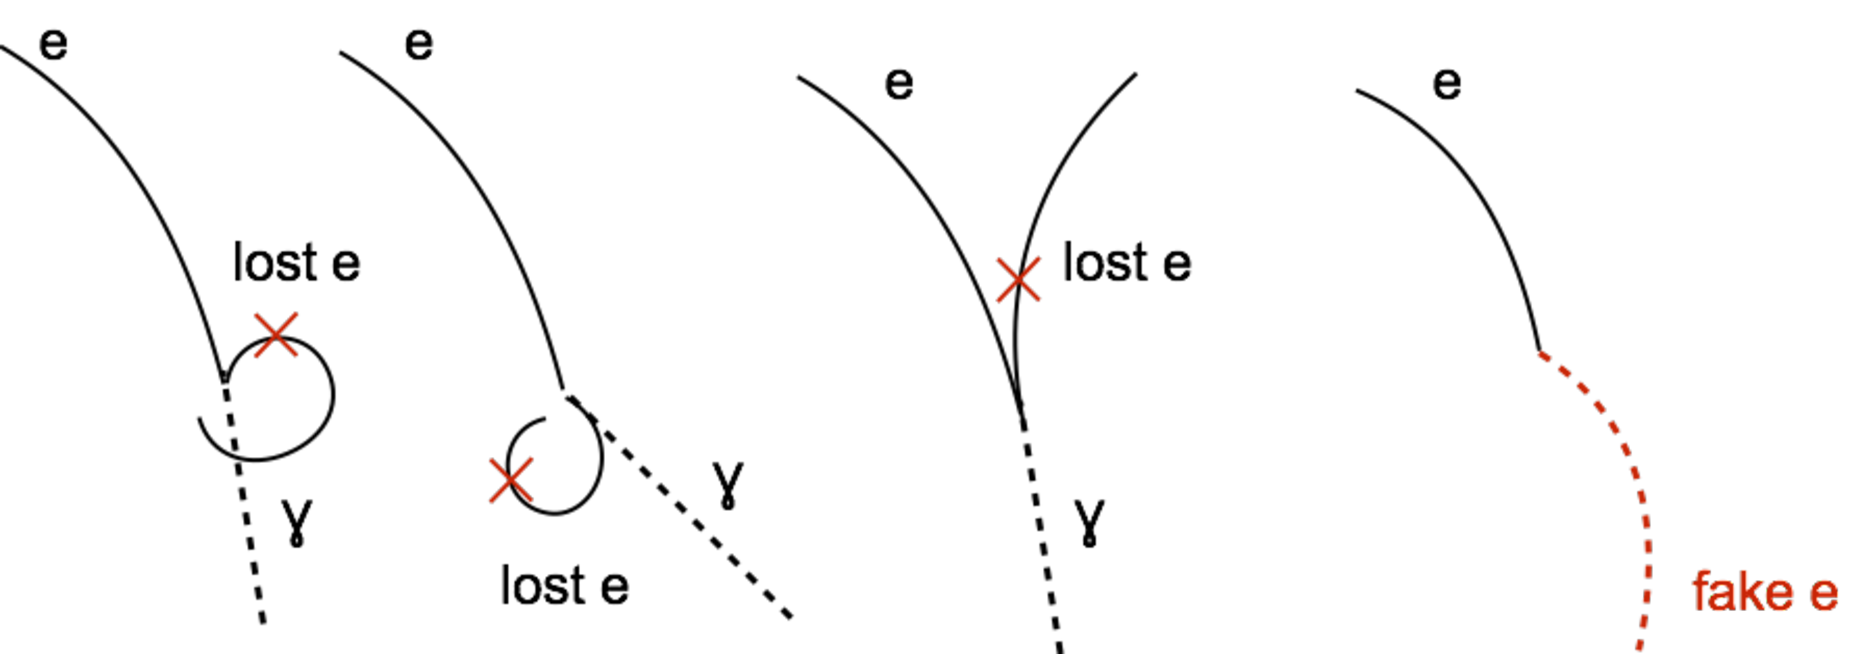
\includegraphics[width=\textwidth]{Figures/PhotonFakeDiagJustDiagTEST.pdf}
    \end{center}


}

\fr{ Composition of $Z\to ee$ background, $e + \gamma$ events } {

    \begin{itemize}
        \item Select events having 1 electron and 1 photon (reco)
        \item Split these events by their truth content
    \end{itemize}

    \bc
        \column{0.5\textwidth}

        \vspace{5mm}

        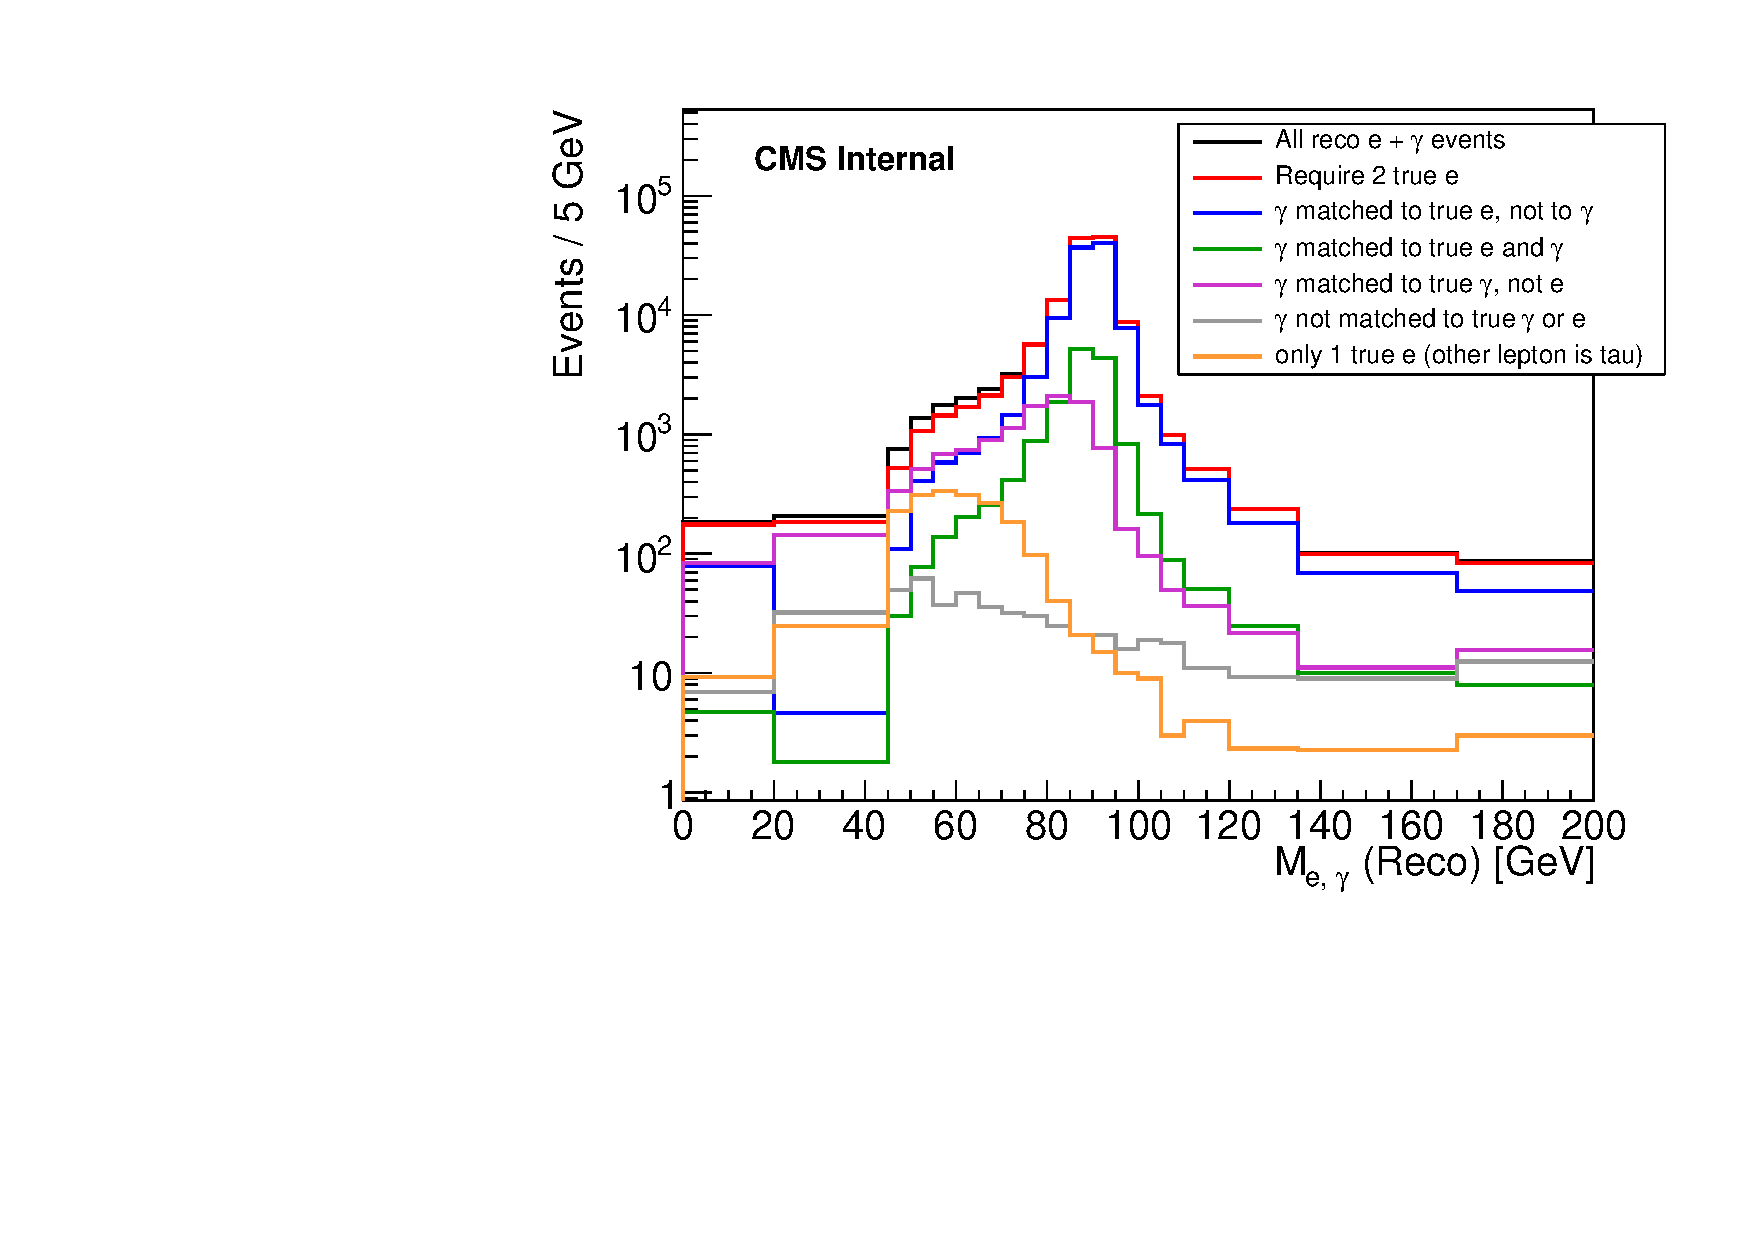
\includegraphics[width=\textwidth]{Plots/DYJetsToLL_1el1ph_truthComp.pdf}

        \column{0.5\textwidth}

        \scriptsize 

        Photon matched to true photon, break down by \pt of subleading truth lepton

        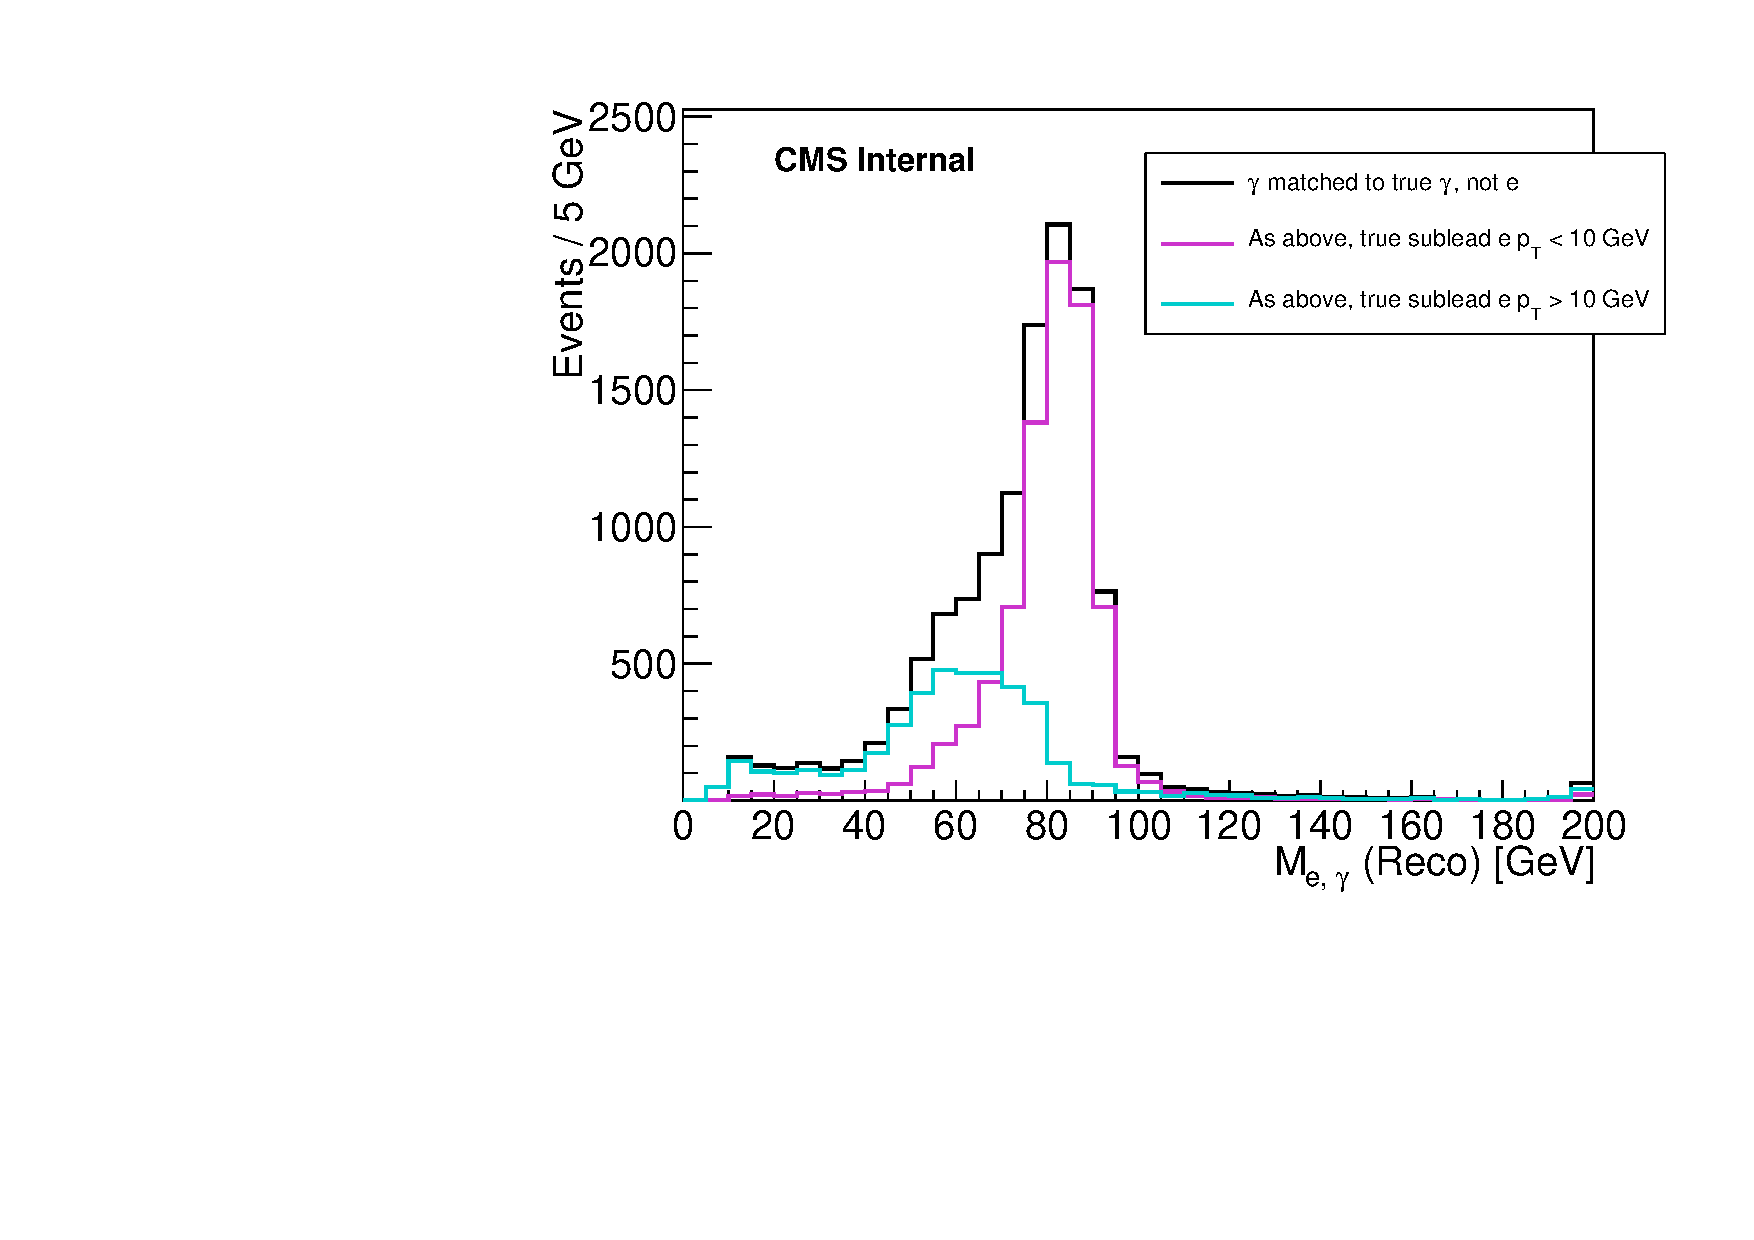
\includegraphics[width=\textwidth]{Plots/DYJetsToLL_1el1ph_truthCompRealPhotons.pdf}

    \ec

}

\fr{ Composition of $Z\to ee$ background, $e + \gamma$ events } {

    \begin{itemize}
        \item Look at events as in the previous slide where the reco photon is matched to a true photon
        \item Split by the mother of the true photon
    \end{itemize}

    \bc
        \column{0.5\textwidth}

        \scriptsize

        DYJetsToLL sample -- most events are FSR

        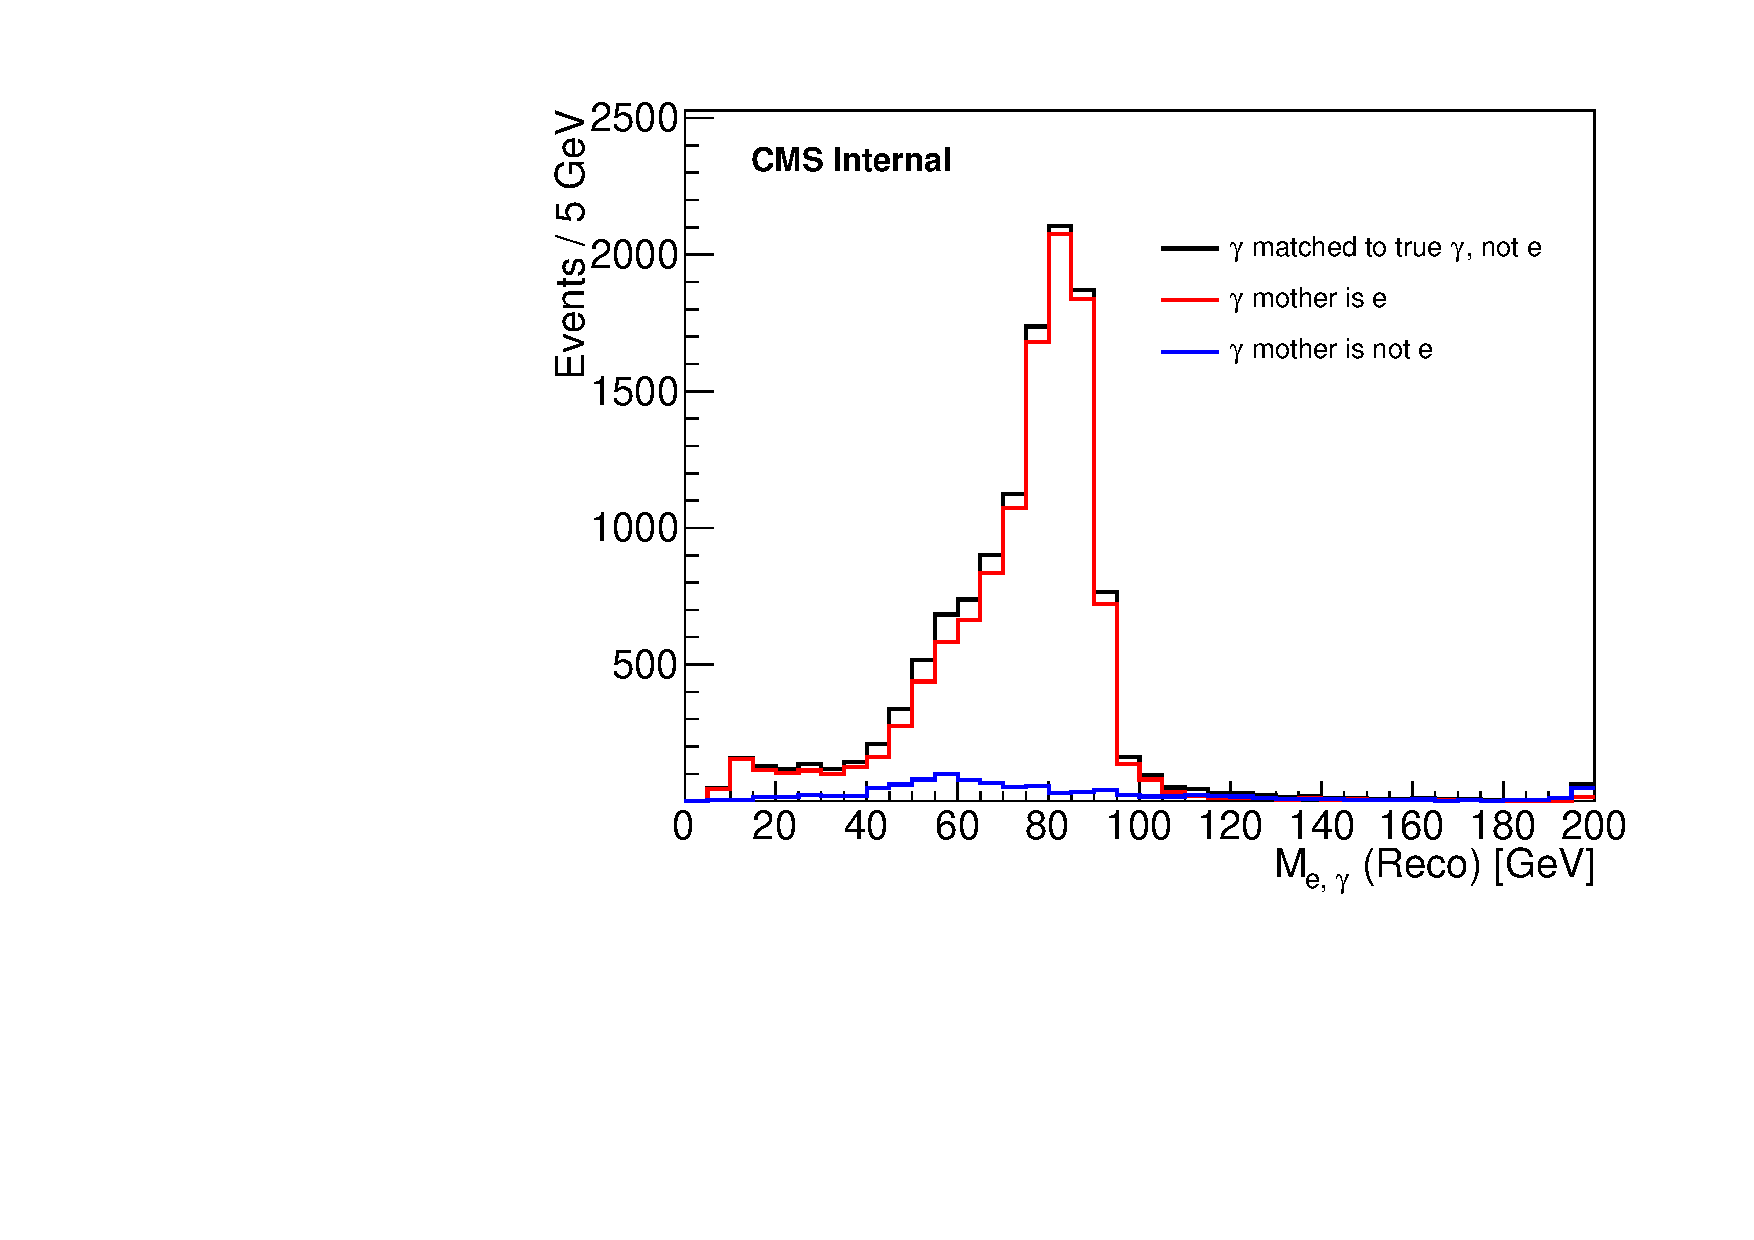
\includegraphics[width=\textwidth]{Plots/DYJetsToLL_1el1ph_truthCompRealPhotonsMatching.pdf}

        \column{0.5\textwidth}

        \scriptsize

        Zg sample -- most events are ISR

        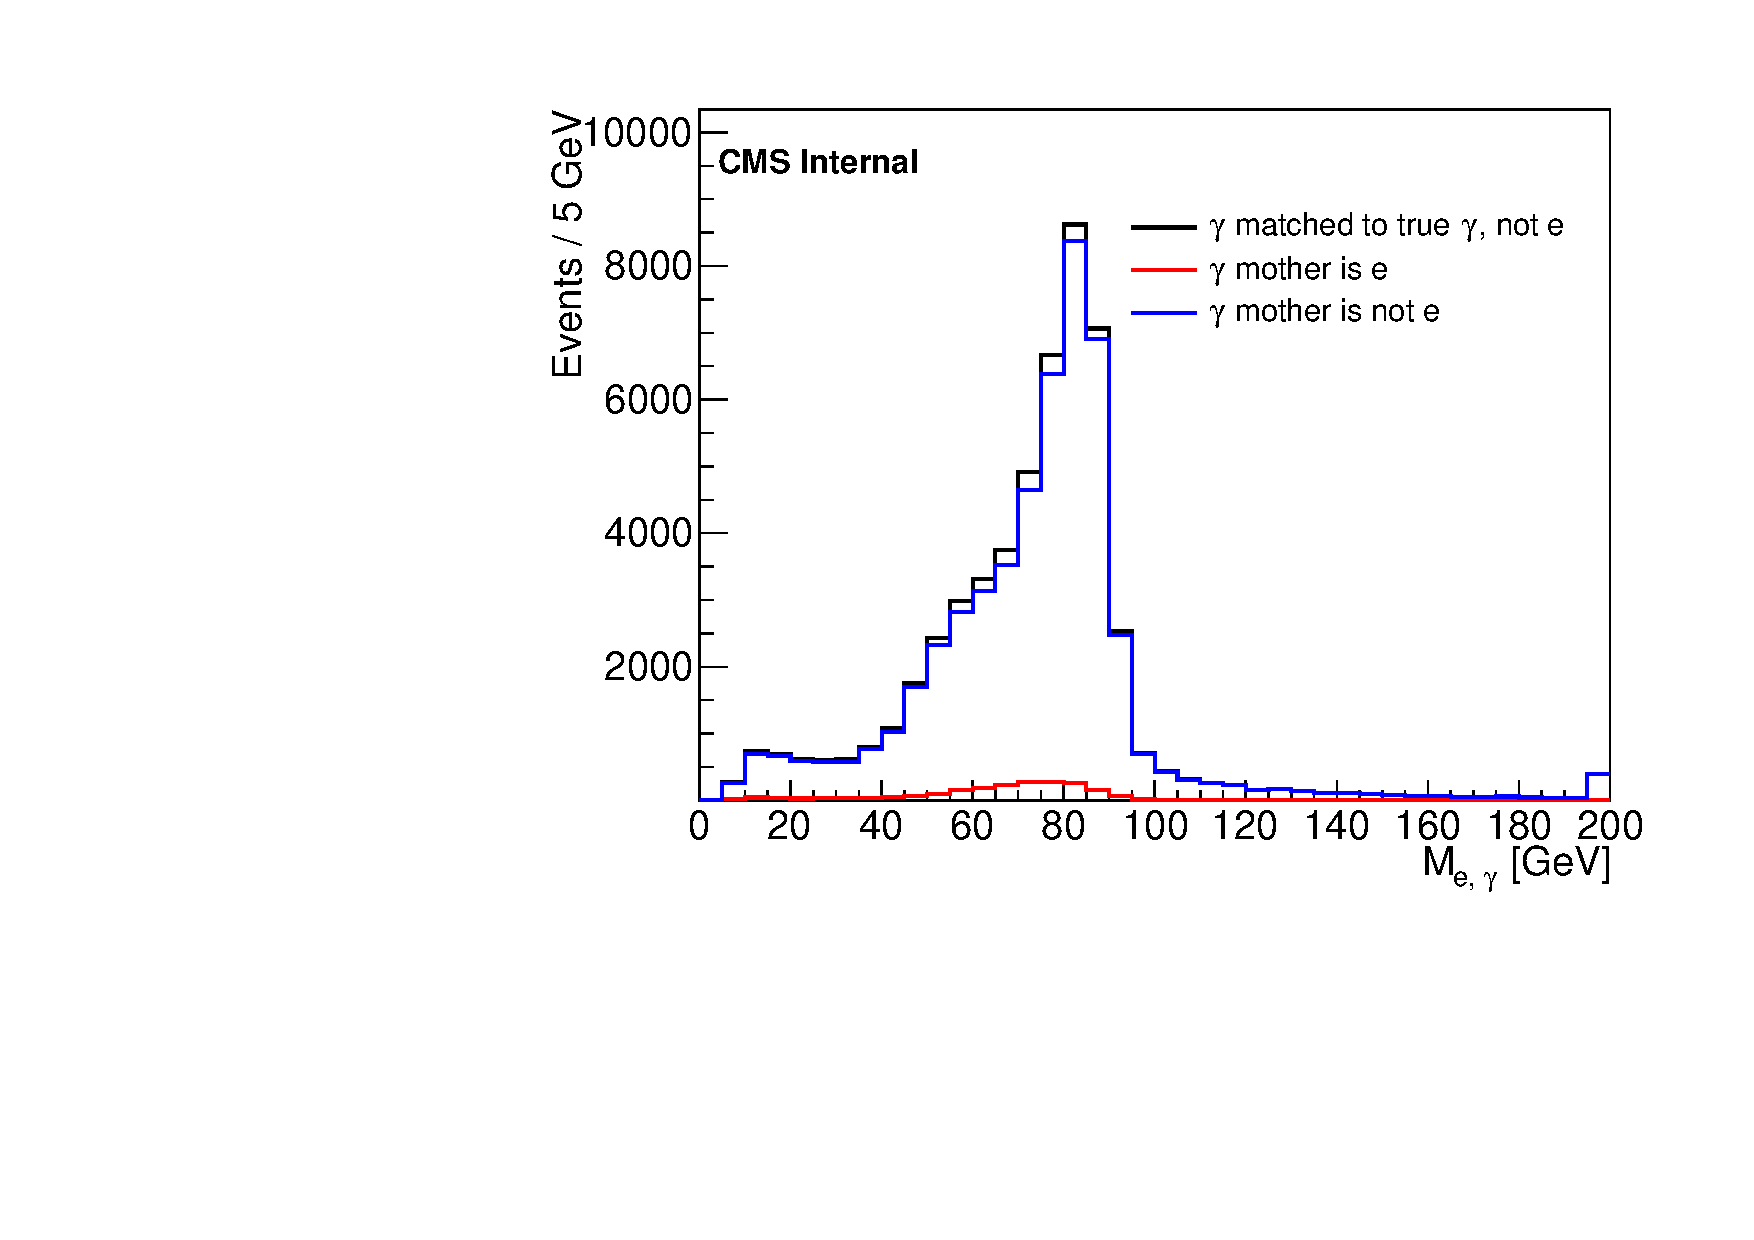
\includegraphics[width=\textwidth]{Plots/DYJetsToLL_1el1ph_truthCompRealPhotonsMatchingZg.pdf}

    \ec

}

\fr{ Estimating $Z \to ee$ background } {

    \begin{itemize}
        \item Derive a relative fake factor using $Z\to ee$ events where the electron passes the nominal ID, or passes the photon ID (mutually exclusive)
    \end{itemize}
    
    \begin{center}
        For all true $Z\to ee$ events the possible reonstructed states are
        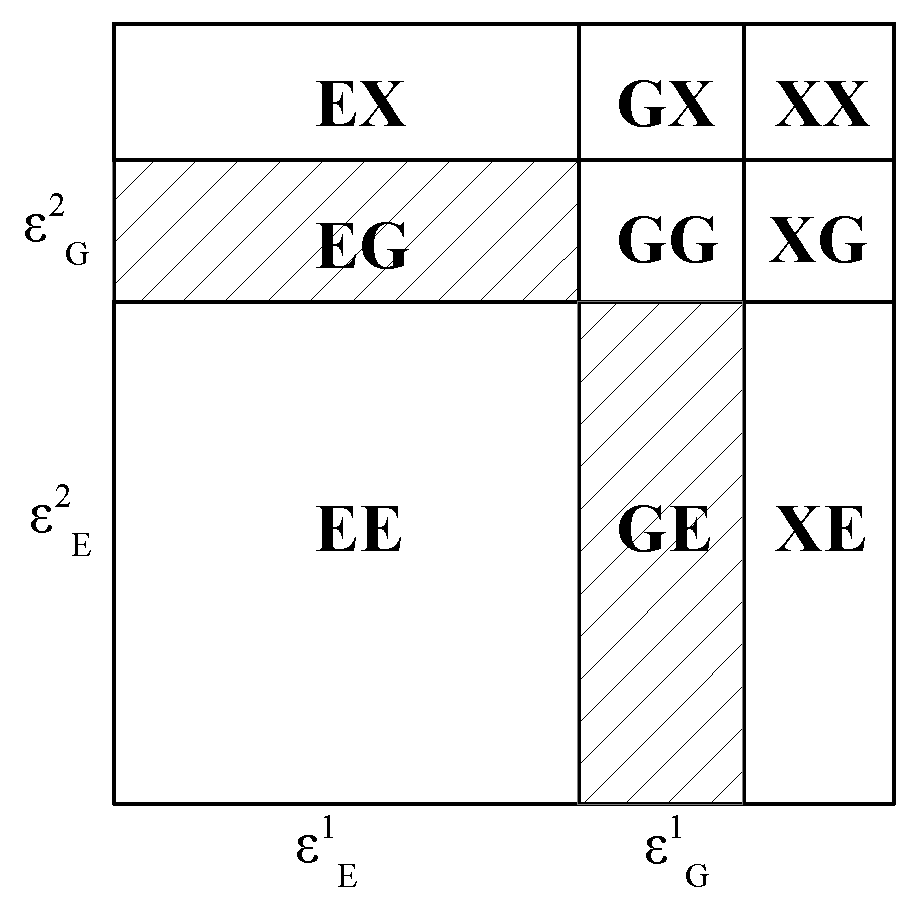
\includegraphics[width=0.5\textwidth]{Figures/ElectronPhotonBox.pdf}
    \end{center}


}

\fr{ Probability to reconstruct a photon fake } {


    \begin{itemize}
        \item $\epsilon_{E,G}^{i}$ represents the rate to reconstruct an electron or photon (E, G) for true electron $i$
        \item $\epsilon$ may depend on kinematic variables ($p_{T}$, $\eta$, ...).  Keep $\epsilon^{1}$ and $\epsilon^{2}$ separate for this reason
    \end{itemize}

    The number of electron plus photon events is given by,
    \begin{equation}
        N_{EG} = N_{Z} \left( \epsilon_{E}^{1}\epsilon_{G}^{2} + \epsilon_{G}^{1}\epsilon_{E}^{2}\right) 
    \end{equation} 
    And the number of two electron events is,
    \begin{equation}
      N_{EE} = N_{Z} \epsilon_{E}^{1}\epsilon_{E}^{2}
    \end{equation} 
      Plug in to remove $N_{Z}$
    \begin{equation}
    \frac{N_{EG}}{N_{EE}} = \frac{\epsilon_{G}^{1}}{\epsilon_{E}^{1}} + \frac{ \epsilon_{G}^{2}}{\epsilon_{E}^{2}} 
    \end{equation} 

    We therefore need $N_{EE}$ and the ratio of the electron reconstruction efficiency to the photon reconstruction efficiency (fake factor)
      
}

\fr{ Fake factor determination } {

    \begin{itemize}     
        \item Select events with at least one tag electron
        \begin{itemize}
            \item \pt $>$ 30 GeV, trigger matched, pass trigger MVA ID
        \end{itemize}
        \item Probes are electrons passing the MVA ID or photons that pass the nominal loose ID
        \item In di-electron events both electrons are used if they both pass the tag selection
        \begin{itemize}
            \item Electrons : \pt $>$ 15 GeV, pass MVA ID
            \item Photons : \pt $>$ 15 GeV, pass loose ID
        \end{itemize}
        \item Require the di-object mass to be within 5 GeV of the Z mass
        \item apply additional electron veto ( MVA ID, \pt $>$ 10 GeV )
        \item fake factor is the ratio of the number of probe photons to probe electrons (binned in $\pt$, $\eta$ )
    \end{itemize}
        

}

\fr{ Example -- mid \pt } {

    \bc
        \column{0.5\textwidth}

        Probe electrons

        \includegraphics[width=\textwidth]{Plots/{m_tagprobe_probeEl_pt_40_45_eta_-2.500000_2.500000}.pdf}

        \column{0.5\textwidth}

        Probe photons

        \includegraphics[width=\textwidth]{Plots/{m_tagprobe_probePh_pt_40_45_eta_-2.500000_2.500000}.pdf}

    \ec
    

}

\fr{ Example -- low \pt } {

    \begin{itemize}
        \item W background is an issue in the electron + photon selecton at low pt
        \item MC subtraction may not be sufficient because statistics are poor in the W MC
    \end{itemize}

    \bc
        \column{0.5\textwidth}

        Probe electrons

        \includegraphics[width=\textwidth]{Plots/{m_tagprobe_probeEl_pt_15_20_eta_-2.500000_2.500000}.pdf}

        \column{0.5\textwidth}

        Probe photons

        \includegraphics[width=\textwidth]{Plots/{m_tagprobe_probePh_pt_15_20_eta_-2.500000_2.500000}.pdf}

    \ec
    
}

\fr{ 1D $\pt$, $\eta$ results } {

    Observe a large difference between simulation and data.  Needs to be checked.

    \bc
        \column{0.5\textwidth}

        Fake factor vs \pt

        \includegraphics[width=\textwidth]{Plots/{TAndPPtCompare}.pdf}

        \column{0.5\textwidth}

        Fake factor vs $\eta$

        \includegraphics[width=\textwidth]{Plots/{TAndPEtaCompare}.pdf}

    \ec

}

\fr{ Sanity check } {

    \bc
        \column{0.5\textwidth}

        Comparison after applying \pt fake factor

        \includegraphics[width=\textwidth]{Plots/{FFComparePtPt}.pdf}

        \column{0.5\textwidth}

        Comparison after applying $\eta$ fake factor

        \includegraphics[width=\textwidth]{Plots/{FFCompareEtaEta}.pdf}

    \ec

}

\fr{ Is a 1D binning sufficient? } {

    A 2D binning is prefered

    \bc
        \column{0.5\textwidth}

        Comparison after applying $\eta$ fake factor

        \includegraphics[width=\textwidth]{Plots/{FFComparePtEta}.pdf}

        \column{0.5\textwidth}

        Comparison after applying \pt fake factor

        \includegraphics[width=\textwidth]{Plots/{FFCompareEtaPt}.pdf}

    \ec


}

\fr{ 2D fake factor } {

    Must widen the bins to have sufficient statistics

    \begin{center}
        \includegraphics[width=0.7\textwidth]{Plots/{FFRessultPtEta}.pdf}
    \end{center}

}

\fr{ Test in 2 photon selection } { 

    \begin{itemize}
        \item Compare $M_{l \gamma\gamma}$ between nominal MC and MC with FF applied
        \item Fairly good agreement is observed
    \end{itemize}

    \begin{center}
        \includegraphics[width=0.7\textwidth]{Plots/{FFCompareMlgg}.pdf}
    \end{center}
}

\fr{ Summary, To do } {


    \begin{itemize}
        \item Developed a basic method for determining the background from fake electrons
        \item Similar to other methods used, but does not rely on a looser photon denominator
        \item Next steps : 
        \begin{itemize}
            \item Apply method to data
            \item A concern is the level of background in the electron+photon selection at low \pt
            \item Plan to present at photon fakes working meeting
        \end{itemize}
    \end{itemize}

}

\fr{ } {

    \[
        A_{W\gamma\gamma} = \frac{N_{MC}^{gen, fiducial}}{N_{MC}^{gen, total}}
    \]

    \[
        C_{W\gamma\gamma} = \frac{N_{MC}^{reco}}{N_{MC}^{gen, fiducial}} \frac{\epsilon^{data}}{\epsilon^{MC}}
    \]
}



\end{document}

